\documentclass{article}
\usepackage{enumerate}
\usepackage{amsmath}
\usepackage{amssymb}
\usepackage{graphicx}
\usepackage{subfigure}
\usepackage{geometry}
\def\degree{${}^{\circ}$}
\geometry{left=3.0cm,right=3.0cm,top=3.0cm,bottom=4.0cm}
\begin{document}

\section*{Problem 1.}
	Suppose the direction to the sky to be the positive direction.
	When the ball goes upwards,
	$$a=\frac{dv}{dt}=-g-\frac{k}{m}v$$
	$$\frac{dv}{g+\frac{k}{m}v}=-dt$$
	Do integral on both side,
	$$\int_{v_0}^v\frac{1}{g+\frac{k}{m}v}dv=-\int_0^tdt$$
	$$\frac{m}{k}ln\frac{mg+kv}{mg+kv_0}=-t$$
	When $v=0$,
	$$t_{max}=\frac{m}{k}ln\frac{mg+kv_0}{mg}$$
	$$\frac{mg+kv}{mg+kv_0}=e^{-\frac{kt}{m}}$$
	$$v=\frac{dh}{dt}=\frac{(mg+kv_0)e^{-\frac{kt}{m}}}{k}-\frac{mg}{k}$$
	Do integral on both side,
	$$\int_0^hdh=\int_0^t\left(\frac{(mg+kv_0)e^{-\frac{kt}{m}}}{k}-\frac{mg}{k}\right)dt$$
	$$h=\left[\frac{-m(mg+kv_0)e^{-\frac{kt}{m}}}{k^2}-\frac{mg}{k}t\right]_0^t
	=\frac{m(mg+kv_0)}{k^2}(1-e^{-\frac{kt}{m}})-\frac{mgt}{k}$$
	When $t=t_{max}$,	
	$$h_{max}=\frac{mv_0}{k}-\frac{m^2g}{k^2}ln\frac{mg+kv_0}{mg}$$
	Similarly, when the ball go downwards,
	$$\int_{0}^v\frac{1}{g+\frac{k}{m}v}dv=-\int_{t_{max}}^tdt$$
	$$\frac{m}{k}ln\frac{mg+kv}{mg}=-t+t_{max}$$
	$$\frac{mg+kv}{mg}=e^{-\frac{k(t-t_{max})}{m}}$$
	$$v=\frac{dh}{dt}=\frac{mge^{-\frac{k(t-t_{max})}{m}}}{k}-\frac{mg}{k}$$
	Do integral on both side,
	$$\int_{h_{max}}^hdh=\int_{t_{max}}^t\left(\frac{mge^{-\frac{k(t-t_{max})}{m}}}{k}-\frac{mg}{k}\right)dt$$
	$$h=h_{max}+\left[\frac{-m^2ge^{-\frac{k(t-t_{max})}{m}}}{k^2}-\frac{mg}{k}t\right]_{t_{max}}^t
	=\frac{m^2g}{k^2}(1-e^{-\frac{kt}{m}}\frac{mg+kv_0}{mg})+
	\frac{m(v_0-gt)}{k}$$
\section*{Problem 2.}
	Suppose the direction to the sky to be the positive direction.
	$$g(h)=\frac{dv}{dt}=\frac{dv}{dh}\cdot\frac{dh}{dt}=-vdv=\frac{g_0R^2}{(R+h)^2}$$
	Do integral on both side,
	$$-\int_0^vvdv=\int_H^h\frac{g_0R^2}{(R+h)^2}dh$$
	$$-\frac{1}{2}v^2=\left[-\frac{g_0R^2}{R+h}\right]_H^h
	=g_0R^2\left(-\frac{1}{R+h}+\frac{1}{R+H}\right)$$
	$$v=\sqrt{\frac{2g_0R^2(H-h)}{(R+H)(R+h)}}$$
	When $h=0$,
	$$v_m=\sqrt{\frac{2g_0R^2(H-h)}{(R+H)(R)}}$$
	$$v=-\frac{dh}{dt}=\sqrt{\frac{2g_0R^2(H-h)}{(R+H)(R+h)}}$$
	$$\sqrt{\frac{(R+H)(R+h)}{2g_0R^2(H-h)}}dh=-dt$$
	Do integral on both side,
	$$\sqrt{\frac{R+H}{2g_0R^2}}\int_H^0\sqrt{\frac{R+h}{H-h}}dh=-\int_0^Tdt$$
	\begin{align*}
	T&=-\sqrt{\frac{R+H}{2g_0R^2}}\left[(h-H)\sqrt{\frac{R+h}{H-h}}+(R+H)\arcsin\sqrt{\frac{R+h}{R+H}}\right]_H^0\\
	&=-\sqrt{\frac{R+H}{2g_0R^2}}\left[-H\sqrt{\frac{R}{H}}+(R+H)\arcsin\sqrt{\frac{R}{R+H}}-(R+H)\frac{\pi}{2}\right]\\
	&=\sqrt{\frac{R+H}{2g_0R^2}}\left[\sqrt{RH}+(R+H)\left(\frac{\pi}{2}-\arcsin\sqrt{\frac{R}{R+H}}\right)\right]
	\end{align*}
	
\section*{Problem 3.}
	\begin{enumerate}[(a)]
	\item
		$$x(t)=\sqrt{B^2+C^2}\sin\left(\omega_0t+\arctan\frac{B}{C}\right)$$
		$$A=\sqrt{B^2+C^2}$$
		$$\varphi=\arctan\frac{B}{C}$$
	\item
		$$x(0)=x_0=A\cos\varphi$$
		$$v(0)=x'(0)=v_0=-\omega A\sin\varphi$$
		$$A^2\cos^2\varphi+A^2\sin^2\varphi
		=x_0^2+\frac{v_0^2}{\omega_0^2}$$
		$$A=\sqrt{x_0^2+\frac{v_0^2}{\omega_0^2}}$$
		$$\frac{v_0}{x_0}=-\omega_0\tan\varphi$$
		$$\varphi=\arctan\left(-\frac{v_0}{\omega_0x_0}\right)$$
	\end{enumerate}
	
\section*{Problem 4.}
	Suppose the direction to the ground to be the positive direction and the ground to be the frame of reference.
	$$h(t)=A\cos(\omega_0t+\varphi)$$
	$$v(t)=h'(t)=-\omega_0A\sin(\omega_0t+\varphi)$$
	$$a(t)=v'(t)=-\omega_0^2A\cos(\omega_0t+\varphi)$$
	The block on the platform is always in contact with the platform when $a(t)\leqslant g$ always holds.
	$$-\omega_0^2A\cos(\omega_0t+\varphi)\leqslant g$$
	$$(\omega_0)_{max}=\sqrt{\frac{g}{A}}$$
	
\section*{Problem 5.}
	$$F=-(k\delta x+\rho gS\delta x)=-(k+\rho gS)\delta x$$
	$$\omega_0=\sqrt{\frac{k}{m}}=\sqrt{\frac{k+\rho gS}{m}}$$
	Suppose that at the equilibrium position, $y=a$\\
	$$mg=k(a-\frac{1}{2}h-l_0)+\rho gS(a+\frac{1}{2}h-H)$$
	$$a=\frac{mg+k(\frac{1}{2}h+l_0)+\rho gS(H-\frac{1}{2}h)}{k+\rho gS}$$
	$$A=|a-y_0|=\left|\frac{mg+k(\frac{1}{2}h+l_0)+\rho gS(H-\frac{1}{2}h)}{k+\rho gS}-y_0\right|$$
	$$y=a+A\sin(\omega_0+\varphi)$$
	$$y=\frac{mg+k(\frac{1}{2}h+l_0)+\rho gS(H-\frac{1}{2}h)}{k+\rho gS}+
	\left(\frac{mg+k(\frac{1}{2}h+l_0)+\rho gS(H-\frac{1}{2}h)}{k+\rho gS}-y_0\right)
	\cos(\sqrt{\frac{k+\rho gS}{m}}t)$$
\section*{Problem 6.}
	The net momentum of the system always equal to zero, so the centroid of the system remains the same position.\\
	Suppose the distance between the centroid and $m_1$, $m_2$ be $l_1$, $l_2$\\
	\begin{eqnarray*}
		\left\{
		\begin{array}{l}		
			m_1l_1=m_2l_2\\
			l_1+l_2=l_0\\
		\end{array}
		\right.\Longrightarrow
		\left\{
		\begin{array}{l}		
			l_1=\frac{m_2}{m_1+m_2}l_0\\
			l_2=\frac{m_1}{m_1+m_2}l_0\\
		\end{array}
		\right.
	\end{eqnarray*}	 
	Then the spring can be divided into two separate systems at the centroid point.\\
	On both sides of the centroid, there is a harmonic
oscillator, and we know that,\\
	$$kl_0=k_1l_1=k_2l_2$$
	$$k_1=\frac{m_1+m_2}{m_2}k,\ k_2=\frac{m_1+m_2}{m_1}k$$
	$$T_1=2\pi\sqrt{\frac{m_1}{k_1}}=2\pi\sqrt{\frac{m_1m_2}{k(m_1+m_2)}}$$
	$$T_2=2\pi\sqrt{\frac{m_2}{k_2}}=2\pi\sqrt{\frac{m_1m_2}{k(m_1+m_2)}}$$
	As $T_1=T_2$, the whole system is under one harmonic
oscillator, and the natural angular frequency,
	$$\omega_0=\frac{2\pi}{T}=\sqrt{\frac{k(m_1+m_2)}{m_1m_2}}$$
\section*{Problem 7.}
	\begin{eqnarray*}
		\left\{
		\begin{array}{l}		
			\delta h_1=\delta l\sin\alpha\\
			\delta h_2=\delta l\sin\beta\\			
		\end{array}
		\right.\Longrightarrow
		\delta h=\delta l(\sin\alpha+\sin\beta)
	\end{eqnarray*}	 
	$$P=\rho g\delta h=\rho g(\sin\alpha+\sin\beta)\delta l$$
	Suppose the radius of the tube to be $r$,
	$$F_{tube}=-PS_1\sin\alpha=-PS_2\sin\beta=-P\pi r^2=-\rho g(\sin\alpha+\sin\beta)\pi r^2\delta l$$
	$$k=\rho g(\sin\alpha+\sin\beta)\pi r^2$$
	$$\omega_0=\sqrt{\frac{k}{m}}=\sqrt{\frac{\rho g(\sin\alpha+\sin\beta)\pi r^2}{\rho\pi r^2l}}=\sqrt{\frac{g(\sin\alpha+\sin\beta)}{l}}$$
\section*{Problem 8.}
	$$F=q(E+v\times B)$$
	$$a=\frac{F}{m}=-\frac{qE_0}{m}\hat{n_x}+\frac{qB_0}{m}v_z\hat{n_y}-\frac{qB_0}{m}v_y\hat{n_z}$$
	$$\frac{a_y}{a_z}=\frac{\frac{dv_y}{dt}}{\frac{dv_z}{dt}}=\frac{dv_y}{dv_z}=-\frac{v_z}{v_y}$$
	$$v_ydv_y=-v_zdv_z$$
	Do integral on both side,
	$$\int v_ydv_y=-\int v_zdv_z$$
	$$\frac{1}{2}v_y^2=-\frac{1}{2}v_z^2+C$$
	$$v_y^2+v_z^2=C=v_{0y}^2$$
	$$v_y=v_{0y}\cos\frac{qB_0}{m}t,\ a_y=\frac{qB_0}{m}v_{0y}\sin\frac{qB_0}{m}t$$
	$$v_z=-v_{0y}\sin\frac{qB_0}{m}t,\ a_z=-\frac{qB_0}{m}v_{0y}\cos\frac{qB_0}{m}t$$
	$$v(t)=\left(v_{0x}-\frac{qE_0}{m}t\right)\hat{n_x}+
	\left(v_{0y}\cos\frac{qB_0}{m}t\right)\hat{n_y}-
	\left(v_{0y}\sin\frac{qB_0}{m}t\right)\hat{n_z}$$
	$$r(t)=\left(v_{0x}t-\frac{qE_0}{2m}t^2\right)\hat{n_x}+
	\left(\frac{m}{qB_0}v_{0y}\sin\frac{qB_0}{m}t\right)\hat{n_y}+
	\left(\frac{m}{qB_0}v_{0y}(\cos\frac{qB_0}{m}t-1)\right)\hat{n_z}$$
	\begin{figure}[h!]
		\centering				
		\subfigure[]{
		\label{Fig.sub.1}
		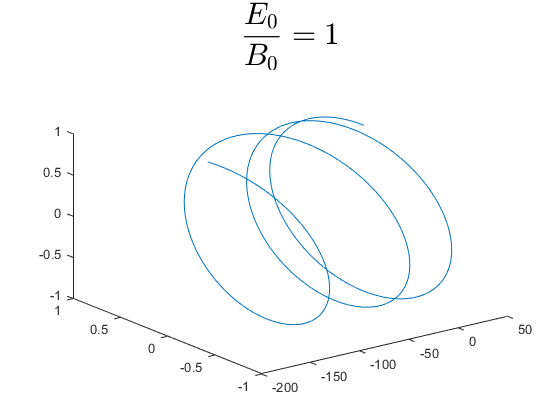
\includegraphics[width=5cm]{p8_1.png}}
		\subfigure[]{
		\label{Fig.sub.2}
		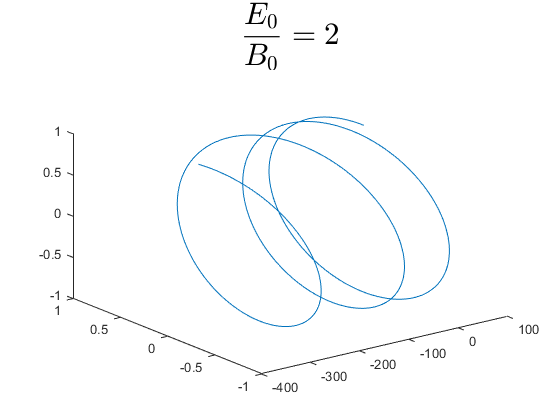
\includegraphics[width=5cm]{p8_2.png}}
		\subfigure[]{
		\label{Fig.sub.3}
		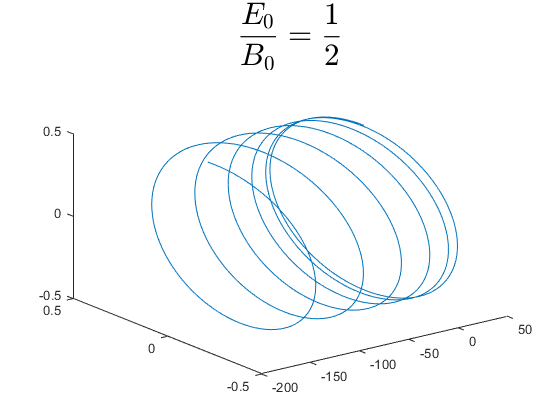
\includegraphics[width=5cm]{p8_3.png}}
		\caption{$r(t)=(t-\frac{1}{2}t^2)\hat{n_x}+\frac{\sin B_0t}{B_0}\hat{n_y}+\frac{\cos B_0t}{B_0}\hat{n_z}$}
		\label{fig-sample}
	\end{figure}
\section*{Problem 9.}
	$$x(t)=D_1e^{-\frac{b}{2m}t}+D_2te^{-\frac{b}{2m}t}$$
	$$x'(t)=\left(D_2-\frac{b(D_1+D_2t)}{2m}\right)e^{-\frac{b}{2m}t}$$
	As $e^{-\frac{b}{2m}t}>0$, $x'(t)=0$ have only one solution $t=\frac{2mD_2-bD_1}{bD_2}$\\
	So $x(t)$ have only one critical point, which means $x(t)=0$ have at most one solution.\\
	So the oscillating mass can pass through the equilibrium position at most once, regardless of initial conditions.
\end{document}
